\chapter{Description du système Client/Serveur : M1}
	
\section{Définition}
	Le système Client/Serveur que nous avons fabriqué à partir du Méta-Modèle HADL
	est très simple. Il est composé d'un client qui envoie une pseudo-requête SQL
	au serveur, qui lui répond.
	
	Le client est très basique. Il permet de saisir une requête, de l'envoyer et
	d'afficher la réponse.
	
	Le serveur lui est plus complexe. Il possède plusieurs fonctionnalités
	internes. Il vérifie que la requête est bien formée, que les éléments demandés
	et l'utilisateur existent et effectue la
	requete.

\section{Analyse}

	\subsection{Client/Serveur}
		C/S est notre système principal. C'est donc une Configuration qui va contenir: 
		\begin{itemize}
			\item le Composant Client.
			\item le Composant Serveur.
			\item le Connecteur RPC qui fait le pont entre Client et Serveur.
			\item un Port Configuration Start\_CS permettant d'activer le système.
			\item un Lien Binding reliant le Port Start\_CS au Client.
			\item plusieur Lien d'Attachement reliant le ClientS, le Serveur et RPC.
		\end{itemize}
		
	\subsection{Client}
		Le Client a un fonctionnement basique : saisi, envoie et reception. C'est
		donc un Composant "Simple". Nous lui fourniront 2 ports :
		\begin{itemize}
			\item Start : permet de lancer le client.
			\item Send-Request : permet d'envoyer un message vers le serveur et de
			recevoir sa réponse.
		\end{itemize}
		
	\subsection{Serveur}
		Le Serveur possède plusieurs fonctionnalités distinctes. C'est donc une
		Configuration va contenir :
		\begin{itemize}
			\item le Composant ConnectionManager : Composant qui gère la bonne syntaxe d'une requete.
			\item le Composant SecurityDB : Composant qui gère la vérification des droits utilisateur.
			\item le Composant DB : Composant contenant la base de données.
			\item le Connecteur ClearenceRequest : pont entre ConnectionManager et SecurityDB.
			\item le Connecteur SecurityQuery : pont entre SecurityDB et DB.
			\item le Connecteur SQLQuery : pont entre ConnectionManager et DB.
			\item Les Lien d'Attachements reliant tous les composants et connecteurs.
			\item Un Lien Binding reliant le Serveur au ConnectionManager.
			\end{itemize}
	
	\subsection{RPC}
		Le Connecteur RPC est très simple et permet de relier Le Client au Serveur.
		
		Il possède 4 rôles et 2 glues permettant de faire transiter un message du
		Client au Serveur et la réponse du Serveur au Client.

\section{Diagrammes}

Nous pouvons voir dans la figure \ref{m1} comment se structure notre système
Client/Serveur. Nous n'y avons pas affiché les attributs des différentes entités pour une meilleur lecture.

	\begin{figure}[!h]
		\centering
		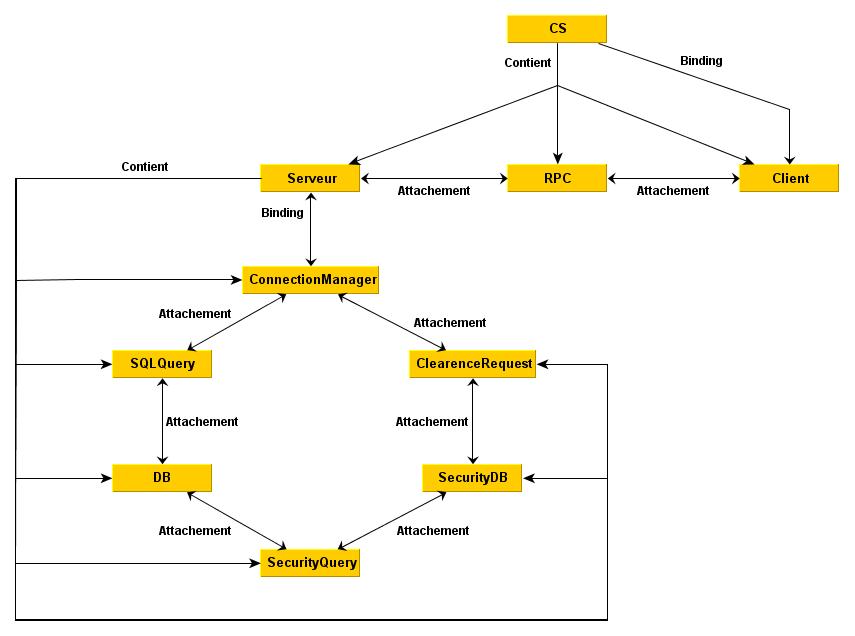
\includegraphics[scale=0.5]{../images/m1}
		\caption{représentation du M1}
		\label{m1}
	\end{figure}
	
Nous pouvons voir dans la figure \ref{zoom_m1} un zoom centré sur le composant
ConnectionManager, où les attributs sont affichés.

	\begin{figure}[!h]
		\centering
		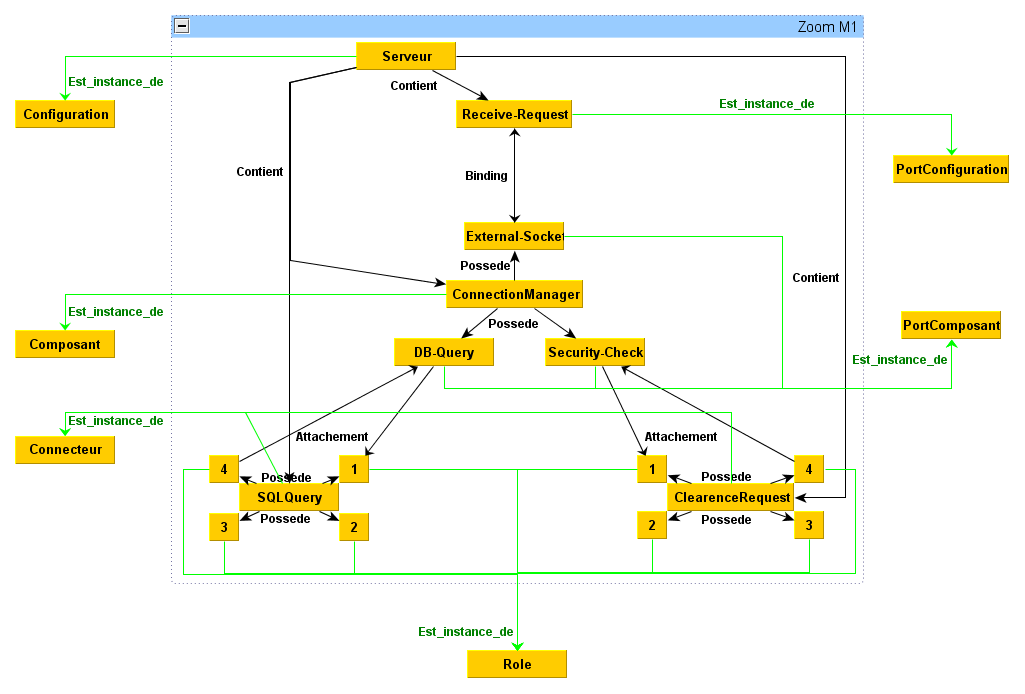
\includegraphics[scale=0.5]{../images/zoom_m1}
		\caption{zoom sur ConnectionManager}
		\label{zoom_m1}
	\end{figure}
	
\clearpage